\documentclass[11pt]{article}
\usepackage[margin=0.85in]{geometry}
\usepackage{amsmath,amssymb,amsthm,mathtools,booktabs,array,graphicx,longtable}
\usepackage[T1]{fontenc}
\usepackage{lmodern,microtype}
\usepackage[colorlinks=true,linkcolor=blue,urlcolor=blue,citecolor=blue]{hyperref}
\newtheorem{theorem}{Theorem}
\newtheorem{proposition}{Proposition}
\newtheorem{corollary}{Corollary}
\newcommand{\E}{\mathbb E}
\newcommand{\Var}{\operatorname{Var}}
\newcommand{\Ree}{\operatorname{Re}}
\newcommand{\one}{\mathbf1}
\setlength{\emergencystretch}{3em}
\setcounter{tocdepth}{1}
\title{Exact controls for homometric scattering:\\proofs and measurement limits}
\author{Scientific completion record for the fixed 63-site construction}
\date{20 October 2026}
\begin{document}
\maketitle

\begin{abstract}
We complete fresh global mean-crossing certificates for three previously
studied Gaussian-motion controls: the original and marginal-preserving
controls each have exactly two simple positive crossings, and the harmonic
control has exactly one. We then impose a stronger control: both homometric
structures receive the same independent Gaussian motion at every site, and
their entire centered displacement covariance matrices agree. Their ensemble
mean intensities agree at every frequency. At a common clean amplitude null,
their first three intensity moments agree exactly, while their fourth moments
differ at every finite positive noise level. A general cumulant selection
theorem identifies the difference as a known diagonal bispectral invariant
times an explicit noise coefficient. For the supplied pair the resulting
fourth-moment gap factors into strictly positive terms. Common Gaussian readout noise and
Poisson counting preserve identifiability. Exact small-noise Hellinger
asymptotics give sharp orders for independent sample requirements:
$\Theta(s^{-10})$ for fixed Gaussian readout or fixed positive photon
background, and $\Theta(s^{-6})$ for zero-background counting. The proofs
concern the specified mathematical models. Publication priority, detector
calibration, and physical realization are not established by this record.
\end{abstract}

\tableofcontents
\clearpage

\section{What is complete and what the claims mean}

The strongest completed statement is that two explicitly specified,
noncongruent point sets remain indistinguishable in their mean diffraction
under one common displacement law, yet have different intensity distributions
at every finite positive noise level. The distinction first appears at the
fourth intensity moment at the selected frequency. This is proved for a
general class of pairs and verified exactly for the fixed 63-site example.

The earlier crossing problem is now closed for all three original controls.
The proof uses exact algebraic coefficients, outward integer intervals,
analytic treatment of the origin, finite interval covers, and bounds on the
entire infinite tail. It does not infer a global root count from a grid.

The measurement analysis establishes both a possible discriminator and a
limitation. Distributional nonidentity survives two specified detector models,
but repeated measurements become expensive as motion tends to zero. This
conclusion follows from probability distances, rather than the numerical size
of an unnormalized moment alone.

\begin{center}
\begin{tabular}{p{0.28\linewidth}p{0.64\linewidth}}
\toprule
Question & Present status\\
\midrule
Mathematical correctness & Explicit analytic proofs plus exact-arithmetic
certificates and separate internal reviews.\\[3pt]
Originality & Established methods and close prior work identified. Priority for
the precise theorem and construction remains unverified.\\[3pt]
Scientific usefulness & Identifiability, a specific statistic, detector
asymptotics, and sharp sample-order limits are proved within stated models.\\[3pt]
Physical validation & No measured data, calibrated instrument, or physical
implementation is supplied here.\\
\bottomrule
\end{tabular}
\end{center}

``Proved'' in this report means a deductive statement from explicit assumptions,
with the computational portions supported by reproducible exact or outward
arithmetic. The reviews were performed by separate AI analysis agents. They
are useful internal checks, not external peer review or verification in a
formal proof assistant. No percentage of infallibility is assigned.

\section{The fixed structures and the common-motion model}
\label{sec:model}

\subsection{Geometry, clean homometry, and the observation frequency}

Set
\[
 \theta=\arcsin\frac1{5\sqrt3},\quad
 \phi=-\arcsin\frac1{8\sqrt3},\quad
 \alpha=\frac{3\theta}{\pi},\quad \beta=\frac{3\phi}{\pi}.
\]
Let $U$ consist of the points $3j+1+(-1)^j\alpha$ and $3j+\epsilon_j$ for
$j=0,\ldots,9$, together with $30$, where
\[
 \epsilon_0=\epsilon_1=0,\qquad
 \epsilon_j=(-1)^j\beta\quad(j=2,\ldots,9).
\]
Define
\[
 V_A=\{0,31,63\},\quad V_B=\{0,32,63\}=63-V_A,
 \qquad A=U+V_A,\quad B=U+V_B.
\]
The bounds $0<\alpha<1/4$ and $-1/4<\beta<0$ show that the listed motif
points are distinct. The motif lies in $[0,30]$, and its three translates
are disjoint in each configuration, so both sets have $n=63$ sites.

For any finite point set $G$, put $F_G(q)=\sum_{r\in G}e^{iqr}$. Sum-set
factorization gives, for every real $q$,
\[
 F_A(q)=F_U(q)F_{V_A}(q),\qquad
 F_B(q)=F_U(q)e^{63iq}\overline{F_{V_A}(q)}.
\]
Consequently $|F_A(q)|^2=|F_B(q)|^2$ for every $q$: the clean structures are
homometric. Choose $q_0=\pi/3$ and write
\[
 z_{Gj}=e^{iq_0r_{Gj}},\qquad M_{G,k}=\sum_j z_{Gj}^k.
\]
Exact phase evaluation gives $M_{A,1}=M_{B,1}=0$. The required algebra uses
\[
 e^{i\theta}=\frac{\sqrt{222}+i\sqrt3}{15},\qquad
 e^{i\phi}=\frac{\sqrt{573}-i\sqrt3}{24},
\]
and the sixth roots of unity associated with integer base positions.
All quantities can therefore be calculated in
$\mathbb Q(\sqrt3,\sqrt{74},\sqrt{191},i)$ with rational coefficients.

\subsection{Identical displacement laws, including the full covariance}

For each configuration, give every site an independent displacement
$\xi_j\sim N(0,\tau^2)$, with the same $\tau^2$ for every site of both
structures. Optional centering gives
\[
 u=P\xi,\qquad P=\mathrm{Id}-\one\one^T/n,\qquad
 \operatorname{Cov}(u)=\tau^2P.
\]
Thus A and B have exactly the same centered covariance matrix. Each marginal
variance is $\tau^2(n-1)/n$ and every off-diagonal covariance is $-\tau^2/n$.
Centering multiplies the field by a phase of modulus one, so it changes no
intensity in any realization.

Let $s=q_0^2\tau^2$ be the raw Gaussian phase variance, and let
$v=\E\|u\|^2/n$ be the centered displacement mean square. Then
\begin{equation}\label{eq:noise-units}
 s=\frac{7\pi^2}{62}v,\qquad
 t=e^{-s/2},\qquad x=e^{-s}=t^2.
\end{equation}
The intensity at the selected frequency has the equivalent representation
\[
 F_G(s)=\sum_{j=1}^n z_{Gj}e^{i\sqrt{s}Z_j},\qquad
 I_G(s)=|F_G(s)|^2,\qquad Z_j\stackrel{\rm iid}{\sim}N(0,1).
\]
In particular, $0\le I_G\le n^2$.

The distinction between $s$ and a standard deviation matters: all powers in
the detector and sampling results below are powers of phase \emph{variance}.
The symbol $x$ in \eqref{eq:noise-units} is an attenuation in $(0,1]$.
The root certificates later use a different, nonnegative coordinate $y$.

\subsection{The mean remains equal at every frequency}

For independent identical displacements with characteristic function
$\psi(q)=\E e^{iq\xi_j}$, separating diagonal and off-diagonal terms gives
\begin{equation}\label{eq:common-mean}
 \E I_G(q)=n+|\psi(q)|^2\bigl(|F_G(q)|^2-n\bigr).
\end{equation}
This exact identity, whose displacement-theory background is established
\cite{Gabrielli2004,Klatt2020}, does not require Gaussianity. Clean homometry
therefore makes the means identical at every frequency. For Gaussian
displacements $|\psi(q)|^2=e^{-q^2\tau^2}$. At $q_0$ the common mean is
$n(1-e^{-s})=n(1-t^2)$.

\section{A general theorem selecting the fourth intensity moment}
\label{sec:general-theorem}

\begin{theorem}[Homometric null with a nonzero diagonal invariant]
Let two collections of $n$ unit complex phases satisfy
\[
 M_{A,1}=M_{B,1}=0,\qquad |M_{A,k}|=|M_{B,k}|\quad(k=2,3,4).
\]
Apply the same independent Gaussian phase variance $s$ at every site.
Define
\[
 D=\Ree\!\left(M_{A,4}\overline{M_{A,2}}^{\,2}\right)
   -\Ree\!\left(M_{B,4}\overline{M_{B,2}}^{\,2}\right).
\]
Then the intensity moments of orders zero through three agree for every
$s\ge0$, and
\begin{equation}\label{eq:general-gap}
 \E I_A^4-\E I_B^4=6\kappa_{40}(t)\kappa_{20}(t)^2D,
\end{equation}
where
\[
 \kappa_{20}=t^4-t^2,\qquad
 \kappa_{40}=t^4(t^2-1)^3(t^6+3t^4+6t^2+6).
\]
If $D\ne0$, the two intensity distributions differ for every finite $s>0$.
\end{theorem}

\begin{proof}
For one random phase $w=e^{i\sqrt{s}Z}$,
\[
 \mu_{ab}=\E(w^a\bar w^b)=t^{(a-b)^2}.
\]
Let $\kappa_{ab}$ be its mixed cumulants, defined by the coefficients of
$\log\E e^{uw+v\bar w}$ near zero. Since $|w|=1$, the generating function
exists there. Deterministic phase multiplication and independence give the
field cumulants
\[
 K_{G,ab}=\kappa_{ab}M_{G,a-b},\qquad
 M_{G,0}=n,\quad M_{G,-k}=\overline{M_{G,k}}.
\]
The single-site cumulants are real and symmetric in $a,b$. The ordinary
second and fourth cumulant identities give
\begin{align*}
 \kappa_{20}&=t^4-t^2,\\
 \kappa_{40}&=t^{16}-4t^{10}-3t^8+12t^6-6t^4\\
 &=t^4(t^2-1)^3(t^6+3t^4+6t^2+6).
\end{align*}

Expand $\E(F_G^p\bar F_G^p)$ by partitions of $p$ labelled positive slots
and $p$ labelled negative slots. A block containing $a$ positive and $b$
negative slots contributes $\kappa_{ab}M_{G,a-b}$. Call $a-b$ its charge.
The charges sum to zero. Any block of charge $\pm1$ vanishes by the null
condition, while a zero-charge block contributes the common structural
factor $n$. The sum of positive charges is at most $p$.

For $p\le3$, every surviving nonzero charge list is a pair $(+2,-2)$ or
$(+3,-3)$, possibly accompanied by zero-charge blocks. Its structural
dependence is through $n,|M_2|^2,|M_3|^2$, which are shared.
For $p=4$, the complete nonzero-charge possibilities are
\[
 \begin{gathered}
 \varnothing;\quad (+2,-2),\ (+3,-3),\ (+4,-4);\\
 (+2,+2,-2,-2);\quad (+4,-2,-2),\ (-4,+2,+2).
 \end{gathered}
\]
The first five types depend only on the shared magnitudes. In the pattern
$(+4,-2,-2)$, all eight slots are used: one block contains the four positive
slots, and two unordered pairs partition the four negative slots. There are
exactly three pairings. This contributes
\[
 3\kappa_{40}\kappa_{02}^2M_4\overline{M_2}^{\,2}.
\]
Its conjugate pattern contributes the complex conjugate. Their sum and A--B
subtraction prove \eqref{eq:general-gap}. For $0<t<1$, $\kappa_{40}<0$ and
$\kappa_{20}^2>0$. Hence a nonzero $D$ makes the fourth moments different.
Bounded random variables with identical laws have identical fourth moments,
which proves nonidentity of the laws.
\end{proof}

The real invariant in this theorem is the real diagonal bispectrum of the
\emph{clean structure} at frequencies $(2q_0,2q_0,-4q_0)$. The bispectrum
and its relation to triple correlations are established concepts
\cite{Jaming2003}. The invariant is third order in clean Fourier amplitudes;
$I^4$ is a fourth intensity moment, equivalently an eighth field moment.
These are different meanings of ``order.'' The theorem is a sufficient
condition. If $D=0$, it does not decide whether higher moments or other
frequencies distinguish the pair.

\section{An exact nonzero gap for the 63-site pair}
\label{sec:instance}

Exact evaluation from the phases in Section~\ref{sec:model} gives
\begin{align*}
 M_{A,2}&=\frac{71}{40}+\frac{413}{40}i\sqrt3,&
 M_{B,2}&=\frac{131}{8}+\frac{171}{40}i\sqrt3,\\
 M_{A,3}&=-1+\frac{1183}{400}i\sqrt3,&
 M_{B,3}&=1-\frac{1183}{400}i\sqrt3,\\
 M_{A,4}&=\frac{123901}{48000}-\frac{470783}{48000}i\sqrt3,&
 M_{B,4}&=\frac{6145}{384}-\frac{173441}{48000}i\sqrt3.
\end{align*}
The magnitudes agree as required, and $|M_{G,2}|^2=129187/400$.
Multiplication gives
\[
 \Ree(M_{A,4}\overline{M_{A,2}}^{\,2})
 =-\frac{455015761}{240000},\qquad
 \Ree(M_{B,4}\overline{M_{B,2}}^{\,2})
 =\frac{455015761}{240000}.
\]
These real quantities are unchanged by a translation, because translation
phases cancel, and by reflection, because reflection conjugates the product.
Their unequal values therefore also prove that A and B are not related by a
translation or reflection.

Substitution into the general theorem yields the central exact identity:
\begin{equation}\label{eq:concrete-gap}
 \boxed{\displaystyle
 \Delta_4(s)=\frac{455015761}{20000}
 x^4(1-x)^5(x^3+3x^2+6x+6)>0,
 \qquad x=e^{-s},\quad 0<s<\infty.}
\end{equation}
The first three raw moments match; consequently the variances and third
central moments match, and the fourth central-moment and fourth-cumulant
differences equal $\Delta_4$.

At the convenient exact point $s=\log2$, so $x=1/2$,
\[
 v=\frac{62\log2}{7\pi^2},\qquad
 \Delta_4=\frac{35946245119}{81920000}
 =438.79693748779296875.
\]
The common variance at this point is $6454387/6400$. The difference in
excess kurtosis is therefore
\[
 \frac{\Delta_4}{(\Var I_G)^2}
 =\frac{35946245119}{83318223091538}
 \simeq 0.00043143317.
\]
The dimensional size of $\Delta_4$ alone is not a measure of classification
accuracy. Standardization and probability-distance bounds are needed.

\subsection{A bounded witness and its precise optimality class}

For $0\le f\le1$, $|\E_Af-\E_Bf|\le d_{\rm TV}(P_A,P_B)$.
Normalize intensity by $y=I/n^2\in[0,1]$ and choose
\[
 f(y)=\frac{1+T_4(2y-1)}2
 =64y^4-128y^3+80y^2-16y+1,
\]
where $T_4(z)=8z^4-8z^2+1$. Since $T_4(\cos\vartheta)=\cos4\vartheta$,
$f$ lies in $[0,1]$. The first three moment differences cancel, giving
\begin{equation}\label{eq:bounded-witness}
 d_{\rm TV}(P_A,P_B)\ge\frac{64\Delta_4(s)}{n^8}>0.
\end{equation}
At $s=\log2$ the right side equals
\[
 \frac{35946245119}{317639398742426880000}
 \simeq1.13166834\times10^{-10}.
\]
This is a conservative lower bound, not an estimate of actual TV.

The factor 64 is optimal among polynomials of degree at most four constrained
to $[0,1]$ throughout the full interval $y\in[0,1]$. Indeed, for any such
polynomial $g$ with leading coefficient $a_4$, let
$p(z)=2g((z+1)/2)-1$. Then $|p|\le1$ on $[-1,1]$ and its leading
coefficient is $a_4/8$. If $a_4>64$, the polynomial
$p-(a_4/64)T_4$ has degree at most three, but alternates strictly in sign at
the five extrema $z_j=\cos(j\pi/4)$, and so has at least four distinct
zeros. This is impossible. Apply the same argument to $-p$ for $a_4<-64$.
Thus $|a_4|\le64$, and equality is attained by $f$.
This argument does not optimize over all bounded functions or all experiments.

\subsection{The unique maximum of this witness gap}

Put $C=455015761/20000$ and view the gap as a polynomial in $x$. Direct
differentiation gives
\[
 \frac{d\Delta_4}{dx}=2Cx^3(1-x)^4H(x),\qquad
 H(x)=12-12x-21x^2-13x^3-6x^4.
\]
The function $H$ is strictly decreasing on $(0,1)$, with $H(0)=12$ and
$H(1)=-40$. It has a unique zero, which is the unique maximum of the gap
and of the bound in \eqref{eq:bounded-witness}. Rational bisection encloses
the zero in an interval of width at most $2^{-160}$, giving
\[
 x_*\simeq0.4718312065944692845,\quad
 s_*\simeq0.7511339705027228761,\quad
 v_*\simeq0.6740797919784131209.
\]
The maximum gap is approximately $445.09685324$, and the maximum value of
the bounded-witness TV lower bound is approximately
$1.14791598\times10^{-10}$. The exact $x_*$ bracket and rational gap
enclosures are certified; the displayed logarithmic conversion to $s_*,v_*$
is descriptive decimal evaluation. No claim about the optimum of full TV,
detector performance, or experimental exposure follows from this maximum.

\subsection{Endpoint behavior and the importance of the stronger control}

The factorization gives
\[
 \Delta_4(s)=\frac{455015761}{1250}s^5+O(s^6)
 \quad(s\downarrow0),\qquad
 \Delta_4(s)\sim\frac{1365047283}{10000}e^{-4s}
 \quad(s\to\infty).
\]
At zero motion both intensities are zero. At infinite phase variance the
independent wrapped Gaussian phases approach uniform phases, producing the
same finite-$n$ random-phasor law for both structures. Equality of those
limits is compatible with strict inequality at every finite positive $s$.

The original graph-dependent controls matched selected marginal properties
within each structure but did not impose the same A--B variance profile.
Here the entire noise law is identical across the two structures. Moreover,
their leading small-noise Gaussian intensity laws are also identical; the
new separation is beyond that leading approximation. Therefore the earlier
constant lower bounds for the graph-dependent controls must not be transferred
to this homogeneous control.

\IfFileExists{figures/homogeneous_fourth_moment_and_sampling.pdf}{
\begin{figure}[tb]
\centering
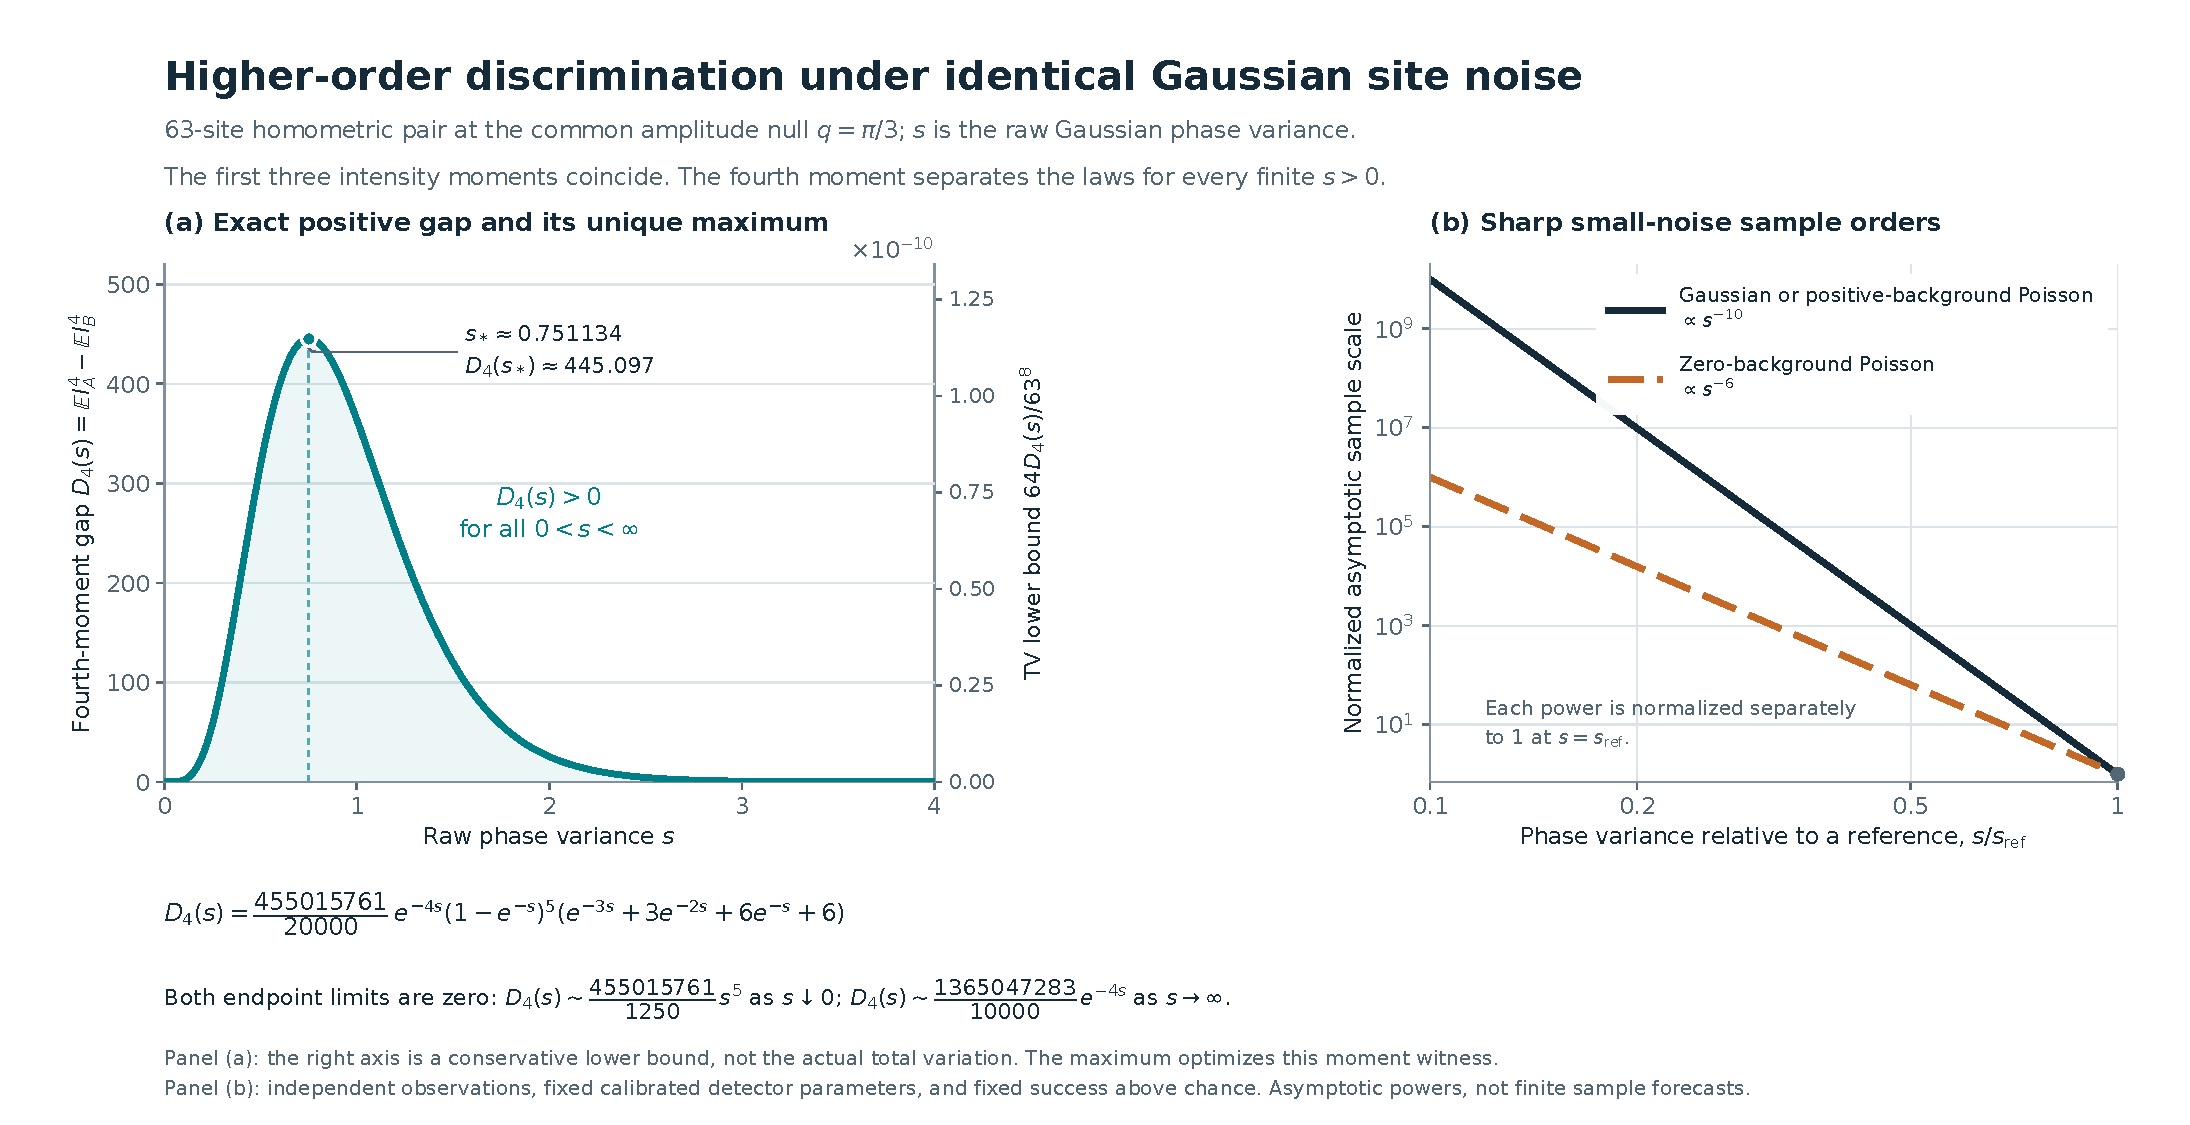
\includegraphics[width=\linewidth]{figures/homogeneous_fourth_moment_and_sampling.pdf}
\caption{Exact homogeneous-control gap and the asymptotic sampling powers.
The TV axis is a conservative lower bound. The normalized sampling curves
show powers only; they do not predict finite sample counts.}
\end{figure}}{}

\section{Common measurement noise and the fifth-power loss of information}
\label{sec:detectors}

This section derives consequences of the homogeneous-control theorem. These
are mathematical measurement models, not experimental validation. The phase
variance is $s>0$, the number of sites is $n=63$, and
\[
 X_s=I_A(s),\qquad Y_s=I_B(s),\qquad 0\le X_s,Y_s\le n^2.
\]
Their first three moments agree exactly. Write
\[
 D_j(s)=\mathbb E X_s^j-\mathbb E Y_s^j,\qquad
 C=\frac{455015761}{20000},\qquad c_5=16C=\frac{455015761}{1250}.
\]
The exact fourth-moment identity gives
\[
 D_4(s)=C e^{-4s}(1-e^{-s})^5
 (e^{-3s}+3e^{-2s}+6e^{-s}+6)>0,
 \qquad D_4(s)=c_5s^5+O(s^6).
\]
The separately computed fifth-moment polynomial satisfies
$D_5(s)=O(s^6)$. This also follows analytically: the scaled intensities
$I_G(s)/s$ tend in every fixed moment to the squared modulus of a complex
Gaussian with common covariance and common pseudocovariance magnitude;
therefore the $s^5$ coefficients of the fifth moments agree. Every moment
is a finite exponential polynomial, so its Taylor expansion has integer
powers. The saved rational calculation verifies all coefficients through
order five of $D_5$ are zero without using this limiting argument.

\subsection{A uniform moment bound}

Let $Z\sim N(0,I_n)$, $P=I-\mathbf1\mathbf1^T/n$, and $U=PZ$.
Centering changes the amplitude by a common phase and leaves intensity
unchanged. At the common clean null, $\sum_i z_i=0$, so
\[
 \left|\sum_i z_i e^{i\sqrt{s}U_i}\right|
 =\left|\sum_i z_i(e^{i\sqrt{s}U_i}-1)\right|
 \le\sqrt{ns}\,\|U\|.
\]
Since $\|U\|^2$ is chi-square with $n-1$ degrees of freedom,
\begin{equation}\label{eq:Bp}
 \mathbb E X_s^p+\mathbb E Y_s^p\le B_p s^p,
 \qquad B_p=2n^p\prod_{j=0}^{p-1}(n-1+2j).
\end{equation}
The identity for the chi-square moment follows by differentiating its
moment generating function $(1-2t)^{-(n-1)/2}$ at zero. This estimate is
deliberately conservative and holds for every $s>0$.

\subsection{Distinction survives common additive noise}

Let $E$ have any fixed distribution with finite fourth absolute moment,
independent of the intensity, and use the same noise law for A and B.
The binomial expansion proves that the first three moments of $X_s+E$
and $Y_s+E$ agree and
\[
 \mathbb E(X_s+E)^4-\mathbb E(Y_s+E)^4=D_4(s)>0.
\]
Thus the measured distributions remain distinct at every finite positive
$s$. This is an identifiability statement; it supplies no uniform practical
accuracy guarantee as the noise level grows or the signal shrinks.

\subsection{Gaussian readout: an exact leading total-variation asymptotic}

Take $E\sim N(0,\sigma^2)$ with fixed $\sigma>0$, and let $g_\sigma$ be its
density. Denote total variation by $d_{\rm TV}(P,Q)=\tfrac12\|p-q\|_1$
when densities exist. Taylor's theorem with an integral remainder gives,
in $L^1(\mathbb R)$,
\[
 p_A-p_B=\frac{D_4(s)}{24}g_\sigma^{(4)}
             -\frac{D_5(s)}{120}g_\sigma^{(5)}+R_s,
 \qquad
 \|R_s\|_1\le\frac{B_6s^6}{720}\|g_\sigma^{(6)}\|_1.
\]
All terms of degree zero through three cancel. Translation invariance of
the $L^1$ norm justifies the remainder bound for all nonnegative input
values, including unbounded Taylor segments. Consequently,
\begin{equation}\label{eq:gaussian-asymptotic}
 d_{\rm TV}(X_s+E,Y_s+E)
 =\frac{c_5}{48}\|g_\sigma^{(4)}\|_1s^5+O(s^6).
\end{equation}
The remainder may depend on the fixed detector parameter $\sigma$.
In particular the distance is of order $s^5$, with a strictly positive
coefficient; this statement concerns total variation, not merely one
selected statistic.

For explicit constants, let $H_k$ be the probabilists' Hermite polynomial.
Then
\[
 \|g_\sigma^{(k)}\|_1
 =\sigma^{-k}\mathbb E|H_k(Z)|\le\frac{\sqrt{k!}}{\sigma^k},
 \qquad Z\sim N(0,1).
\]
The inequality follows from Cauchy--Schwarz and
$\mathbb E H_k(Z)^2=k!$, which follows by repeated Gaussian integration
by parts. Put $a=\sqrt{3-\sqrt6}$, $b=\sqrt{3+\sqrt6}$, and
$\varphi(t)=e^{-t^2/2}/\sqrt{2\pi}$. Splitting at the four roots of
$H_4(t)=t^4-6t^2+3$ and integrating
$(H_3\varphi)'=-H_4\varphi$ yields
\[
 \|g_\sigma^{(4)}\|_1
 =\frac{4\sqrt6}{\sigma^4}\bigl[a\varphi(a)+b\varphi(b)\bigr]>0.
\]

The saved arithmetic supplies rational $A_4,A_5$ such that
\[
 |D_4(s)-c_5s^5|\le A_4s^6,
 \qquad |D_5(s)|\le A_5s^6.
\]
For a polynomial $D_j(s)=\sum_m a_{jm}e^{-ms}$ they are obtained from
$A_j=\sum_m|a_{jm}|m^6/6!$ after the exact lower-order cancellations.
Thus an explicit finite-$s$ error in \eqref{eq:gaussian-asymptotic} is
\begin{equation}\label{eq:gaussian-error}
 s^6\left[
 \frac{A_4\|g_\sigma^{(4)}\|_1}{48}
 +\frac{A_5\|g_\sigma^{(5)}\|_1}{240}
 +\frac{B_6\|g_\sigma^{(6)}\|_1}{1440}\right].
\end{equation}
A simpler all-$s$ upper bound, using a Taylor expansion only through
degree four, is
\[
 d_{\rm TV}(X_s+E,Y_s+E)
 \le\min\left\{1,
 \frac{D_4(s)}{2\sqrt{24}\,\sigma^4}
 +\frac{B_5s^5}{2\sqrt{120}\,\sigma^5}\right\}.
\]

\subsection{Photon counting: strict distinction and fifth-power scaling}

Consider a count $N$ conditional on intensity $I$ with
\[
 N\mid I\sim\operatorname{Poisson}(b+\eta I),
 \qquad b\ge0,\quad\eta>0,
\]
where the background $b$ and gain $\eta$ are fixed and common to the two
hypotheses. The falling factorial $(N)_j=N(N-1)\cdots(N-j+1)$ satisfies
$\mathbb E[(N)_j\mid I]=(b+\eta I)^j$. Hence the first three factorial
moments agree and the fourth differs by $\eta^4D_4(s)>0$. The two count
distributions are therefore distinct for every finite $s>0$.

Let $p_b$ be the Poisson mass function at mean $b$, and let the shift
operator $S$ act by $(Sp)(k)=p(k-1)$ with $p(-1)=0$. Derivatives with
respect to intensity satisfy
\[
 \frac{d^j}{dI^j}p_{b+\eta I}
 =\eta^j(S-\mathrm{Id})^j p_{b+\eta I},
 \qquad \left\|\frac{d^j}{dI^j}p_{b+\eta I}\right\|_1\le(2\eta)^j.
\]
Taylor expansion in the Banach space $\ell^1$ therefore proves
\begin{equation}\label{eq:poisson-asymptotic}
 d_{\rm TV}(N_A,N_B)
 =\frac{c_5\eta^4}{48}\|(S-\mathrm{Id})^4p_b\|_1s^5+O(s^6).
\end{equation}
The leading constant is positive: the generating function of
$(S-\mathrm{Id})^4p_b$ is $(z-1)^4e^{b(z-1)}$, which is not the zero
function. For zero background, $p_0$ is a point mass and the fourth
difference has coefficients $(1,-4,6,-4,1)$, so
\begin{equation}\label{eq:poisson-zero}
 d_{\rm TV}(N_A,N_B)=\frac{c_5\eta^4}{3}s^5+O(s^6).
\end{equation}
An explicit all-$s$ error for this last expression is
\[
 s^6\left[\frac{\eta^4A_4}{3}
 +\frac{2\eta^5A_5}{15}+\frac{2\eta^6B_6}{45}\right].
\]
An all-$s$ upper bound requiring no sixth-order quantities is
\[
 d_{\rm TV}(N_A,N_B)\le\min\left\{1,
 \frac{\eta^4D_4(s)}{3}+\frac{2\eta^5B_5s^5}{15}\right\}.
\]

\subsection{An asymptotically optimal count-parity rule}

In the zero-background model, the difference in even-count probabilities is
\[
 \Pr(N_A\text{ even})-\Pr(N_B\text{ even})
 =\frac12\left(\mathbb E e^{-2\eta X_s}
                   -\mathbb E e^{-2\eta Y_s}\right)
 =\frac{c_5\eta^4}{3}s^5+O(s^6).
\]
The same coefficient occurs in \eqref{eq:poisson-zero}. With equal prior
probabilities and one observation, choosing A on even counts and B on odd
counts therefore has advantage over random guessing asymptotic to the
optimal advantage: the ratio tends to one as $s\downarrow0$.
This is a one-observation asymptotic statement. Its absolute advantage
tends to zero, and the argument does not claim finite-$s$ optimality,
optimality for positive background, or optimality for multiple observations.

\subsection{Sampling and interpretation}

For $m$ independent observations from one unknown configuration with equal
priors, a one-observation TV bound $\delta(s)$ implies
\[
 \Pr(\text{correct})\le\frac{1+\min\{1,m\delta(s)\}}2.
\]
This elementary inequality gives a necessary $\Omega(s^{-5})$ sample bound.
Section~\ref{sec:sampling} improves it to sharp necessary and sufficient
orders using Hellinger distance. Unknown gain, background, noise calibration,
temporal dependence, and changes in the structural model are outside the
stated experiment.


\section{Sharp orders for the number of independent measurements}
\label{sec:sampling}

The preceding total-variation calculation concerns one observation. Repeated
observations require a separate argument: multiplying the one-observation
distance by the number of samples generally loses the correct scaling.
Here that gap can be closed for the stated, fully calibrated detector models.
All limits in this section hold as $s\downarrow0$, with detector parameters
fixed. Define the squared Hellinger distance and the affinity by
\[
 h^2(P,Q)=\int(\sqrt p-\sqrt q)^2,\qquad
 \rho(P,Q)=\int\sqrt{pq}=1-\frac{h^2(P,Q)}2.
\]
Integrals are replaced by sums for count distributions. This convention gives
$0\le h^2\le2$.

\subsection{Common leading moments at every fixed order}

The null condition and the uniform bound in \eqref{eq:Bp} imply
\[
 I_G(s)/s\ \longrightarrow\ J_G
 =\left|i\sum_j z_{Gj}Z_j\right|^2
\]
almost surely and in every fixed moment. Dominated convergence applies because
$I_G(s)/s\le n\|PZ\|^2$, which has every finite moment. The real Gaussian
field has covariance eigenvalues
\[
 \lambda_\pm=\frac{n\pm|M_2|}{2}.
\]
They are the same for A and B. Thus $J_A$ and $J_B$ have the same law as
$\lambda_+ Z_1^2+\lambda_- Z_2^2$ with independent standard normals.
Write $m_k=\mathbb E J_G^k>0$. Each exact intensity moment is a finite sum
of exponentials in $s$, hence is analytic at zero. Therefore, for every fixed
integer $k\ge1$,
\begin{equation}\label{eq:all-leading-moments}
 \mathbb E I_G(s)^k=m_k s^k+O(s^{k+1}),\qquad
 D_k(s)=O(s^{k+1}).
\end{equation}
The exact fourth-moment identity specifies the sharper coefficient
$D_4(s)=c_5s^5+O(s^6)$. Put $R=|M_2|^2=129187/400$. The generating function
\[
 \mathbb E e^{tJ_G}=
 \bigl[1-2nt+(n^2-R)t^2\bigr]^{-1/2}
\]
gives
\begin{equation}\label{eq:m4}
 m_4=24n^4+72n^2R+9R^2>0.
\end{equation}
These facts also justify $D_5=O(s^6)$ and $D_6=O(s^7)$ without assuming
an uncomputed sixth-order symbolic identity.

\subsection{Gaussian readout}

For fixed $\sigma>0$, the squared Hellinger distance between the laws of
$I_A+N(0,\sigma^2)$ and $I_B+N(0,\sigma^2)$ satisfies
\begin{equation}\label{eq:hellinger-gaussian}
 \boxed{\displaystyle
 h^2=\frac{c_5^2}{96\sigma^8}s^{10}+o(s^{10}).}
\end{equation}

\paragraph{Proof.}
Subtract the common mean $\mu(s)=\mathbb E I_G(s)=n(1-e^{-s})=O(s)$ from
both observations; this translation preserves Hellinger distance.
Set $V_G=I_G-\mu$. Then $\mathbb E V_G=0$, $|V_G|\le n^2$, and
$\mathbb E|V_G|^k=O(s^k)$ for every fixed $k$. Equality of the first three
raw moments gives equality of the first three central moments. The fourth
central-moment difference is $D_4$, and the fifth is
$D_5-5\mu D_4=O(s^6)$.

Use the Hilbert norm $\|f\|_{g}^{2}=\int |f(x)|^2/g_\sigma(x)\,dx$.
The translated Gaussian kernels obey the exact identity
\[
 \left\langle g_\sigma(\cdot-u),g_\sigma(\cdot-v)\right\rangle_g
 =e^{uv/\sigma^2}.
\]
It follows either by completing the square or direct Gaussian integration.
All fixed derivatives of these kernels have finite Hilbert norm, uniformly
for $|u|\le n^2$; the derivative norms are an exponential times a polynomial
in $u$. Taylor's theorem in this Hilbert space, through degree five, gives
\[
 \frac{p_{A,s}-p_{B,s}}{s^5}
 \longrightarrow \frac{c_5}{24}g_\sigma^{(4)}
 \quad\hbox{in }L^2(g_\sigma^{-1}dx).
\]
The sixth-order remainder is $O(s^6)$ in that norm by the uniform derivative
bound and $\mathbb E|V_A|^6+\mathbb E|V_B|^6=O(s^6)$.

Jensen's inequality supplies the needed denominator control globally:
\[
 \frac{p_{G,s}(x)}{g_\sigma(x)}
 =\mathbb E\exp\left(\frac{xV_G}{\sigma^2}
                 -\frac{V_G^2}{2\sigma^2}\right)
 \ge \exp\left(-\frac{\mathbb E V_G^2}{2\sigma^2}\right).
\]
This lower bound tends to one, and $p_{G,s}(x)/g_\sigma(x)\to1$ for each
fixed $x$. Hence
\[
 \frac{h^2}{s^{10}}
 =\int\frac{[(p_{A,s}-p_{B,s})/s^5]^2}
                 {(\sqrt{p_{A,s}}+\sqrt{p_{B,s}})^2}
 \longrightarrow
 \frac{c_5^2}{4\cdot24^2}
 \int\frac{(g_\sigma^{(4)})^2}{g_\sigma}.
\]
For completeness, the limit follows from Hilbert-norm convergence of the
numerator, which gives $L^1$ convergence of its weighted square; the extra
factor $g_\sigma/(\sqrt{p_A}+\sqrt{p_B})^2$ is uniformly bounded and tends
pointwise to $1/4$. Differentiating the kernel identity four times in each
variable at zero gives
$\int(g_\sigma^{(4)})^2/g_\sigma=4!/\sigma^8$.
Substitution proves \eqref{eq:hellinger-gaussian}.

\subsection{Photon counting with a fixed positive background}

For fixed $b>0$ and $\eta>0$ in $N\mid I\sim\operatorname{Poisson}(b+\eta I)$,
\begin{equation}\label{eq:hellinger-positive-background}
 \boxed{\displaystyle
 h^2=\frac{c_5^2\eta^8}{96b^4}s^{10}+o(s^{10}).}
\end{equation}

\paragraph{Proof.}
Let $p_\lambda(k)=e^{-\lambda}\lambda^k/k!$ and use the Hilbert norm
$\|f\|_b^2=\sum_k |f(k)|^2/p_b(k)$. Direct summation gives
\[
 \langle p_{b+u},p_{b+v}\rangle_b=e^{uv/b}.
\]
This identity ensures uniform Hilbert bounds for all fixed kernel derivatives
on the compact interval $0\le u\le\eta n^2$. Taylor expansion in intensity
through degree five, the exact lower-moment cancellations, and the sixth
moment bound give
\[
 (p_{A,s}-p_{B,s})/s^5
 \longrightarrow \frac{c_5\eta^4}{24}(S-\mathrm{Id})^4p_b
 \quad\hbox{in }\ell^2(p_b^{-1}).
\]
For every count $k$ and every admissible intensity,
\[
 \frac{p_{b+\eta I}(k)}{p_b(k)}
 =e^{-\eta I}(1+\eta I/b)^k\ge e^{-\eta n^2}.
\]
The mixture ratios tend pointwise to one and have the same positive lower
bound. The argument used for Gaussian readout therefore applies to the
Hellinger denominator. Differentiating the kernel identity gives
\[
 \sum_k\frac{[(S-\mathrm{Id})^4p_b(k)]^2}{p_b(k)}=\frac{4!}{b^4},
\]
which proves the stated coefficient. The assumption $b>0$ is essential;
this formula is not uniform as $b$ tends to zero.

\subsection{Zero-background counting and the four-count event}

At $b=0$ and fixed $\eta>0$ the scaling changes:
\begin{equation}\label{eq:hellinger-zero-background}
 \boxed{\displaystyle
 h^2=\frac{\eta^4c_5^2}{96m_4}s^6+O(s^7).}
\end{equation}

\paragraph{Proof.}
For each fixed count $k$,
\[
 p_{G,s}(k)=\frac{\eta^k}{k!}\mathbb E[I_G^k e^{-\eta I_G}]
 =\frac{\eta^km_k}{k!}s^k+O(s^{k+1}).
\]
For $k=0$, use $m_0=1$. Expanding the remaining exponential and using the
exact equality of moments of orders zero through three shows
$p_{A,s}(k)-p_{B,s}(k)=O(s^5)$ for $k=0,1,2,3$. Their Hellinger contributions
are respectively $O(s^{10}),O(s^9),O(s^8),O(s^7)$.
At $k=4$, the leading probability and the difference are
\[
 p_{G,s}(4)=\frac{\eta^4m_4}{24}s^4+O(s^5),\qquad
 p_{A,s}(4)-p_{B,s}(4)=\frac{\eta^4c_5}{24}s^5+O(s^6).
\]
The second formula uses $D_5=O(s^6)$ and the sixth-moment remainder.
Consequently
\[
 (\sqrt{p_{A,s}(4)}-\sqrt{p_{B,s}(4)})^2
 =\frac{\eta^4c_5^2}{96m_4}s^6+O(s^7).
\]
For $k=5,6$, equation \eqref{eq:all-leading-moments} yields probability
differences $O(s^6),O(s^7)$, so their contributions are $O(s^7),O(s^8)$.
Finally, the entire remaining tail is bounded without any nonuniform series:
\[
 \sum_{k\ge7}(\sqrt{p_{A,s}(k)}-\sqrt{p_{B,s}(k)})^2
 \le\Pr_A(N\ge7)+\Pr_B(N\ge7)
 \le\frac{\eta^7}{7!}(\mathbb E I_A^7+\mathbb E I_B^7)=O(s^7).
\]
Here $\mathbf1_{\{N\ge7\}}\le (N)_7/7!$ supplies the factorial-moment
bound. Summing all contributions proves \eqref{eq:hellinger-zero-background}.

Keeping only the binary indicator $\mathbf1_{\{N=4\}}$ gives the same
leading Hellinger coefficient: its complementary event contributes only
$O(s^{10})$. Thus a frequency estimate of exactly-four-count observations
achieves the optimal sample-order scaling in this limit. This concerns
repeated independent observations, not a claim that four-count events
dominate one-observation total variation at every noise level.

The earlier parity rule illustrates this distinction. Its even-count
probability is $1-\eta ns+O(s^2)$, and its A--B difference is
$(c_5\eta^4/3)s^5+O(s^6)$. If only parity is retained, the two Bernoulli
laws have
\[
 h^2_{\rm parity}=\frac{c_5^2\eta^7}{36n}s^9+O(s^{10}).
\]
Parity is asymptotically optimal for one observation in total variation,
but discarding count magnitude loses information for repeated measurements.

\subsection{From affinity to necessary and sufficient sample orders}

Let $m$ observations be independent conditional on the unknown structure,
with equal prior probabilities for A and B. The optimal success probability
is $(1+d_{\rm TV}(P_s^{\otimes m},Q_s^{\otimes m}))/2$. Direct Cauchy--Schwarz
and $\min(p,q)\le\sqrt{pq}$ give
\[
 1-\rho(s)^m\le d_{\rm TV}(P_s^{\otimes m},Q_s^{\otimes m})
 \le\sqrt{1-\rho(s)^{2m}}.
\]
These bounds and $\rho=1-h^2/2$ prove that, for any fixed target success
$a\in(1/2,1)$, the minimum sample count has order $1/h^2(s)$. More explicitly,
put $r=2a-1$. A necessary sample count is
\[
 m\ge\frac{\log(1-r^2)}{2\log\rho(s)},
\]
and taking the ceiling of $\log(1-r)/\log\rho(s)$ is sufficient for the
optimal likelihood-ratio test. Therefore the sharp orders are
\[
 \boxed{\begin{aligned}
  m_\mathrm{Gaussian}(s)&=\Theta(s^{-10}),&&\sigma>0\text{ fixed},\\
  m_\mathrm{Poisson}(s)&=\Theta(s^{-10}),&&b>0,\ \eta>0\text{ fixed},\\
  m_\mathrm{Poisson}(s)&=\Theta(s^{-6}),&&b=0,\ \eta>0\text{ fixed}.
 \end{aligned}}
\]
With only parity retained in the zero-background case, the sharp order
becomes $\Theta(s^{-9})$. The powers are proved; a universal finite-noise
sample number, an exact optimal prefactor for the minimum sample count,
and an experimental acquisition time are not. Calibration, independent
snapshots, fixed exposure/gain, and the assumed structural model remain
part of the theorem's conditions. Joint limits in $b$, $\eta$, $\sigma$,
or the observation frequency require a separate analysis.



\section{Fresh global crossing proofs for the three earlier controls}
\label{sec:roots}

\subsection{The functions whose roots are counted}

Order each structure's sites by mean position and join pairs separated by less
than $5/2$, holding this graph fixed during the motion. Exact comparison gives a path on 63 vertices with one additional
chord: $(20,22)$ for A and $(41,43)$ for B, using zero-based ordinal indices.
Let $L_G$ be the graph Laplacian, $C_G=L_G^+$ its pseudoinverse,
$\tau_G=\operatorname{tr}C_G$, and
$h_{Gi}=63(C_G)_{ii}/\tau_G$. The three centered covariance coefficients are
\begin{align*}
 K_{H,G}&=63C_G/\tau_G,\\
 K_{0,G}&=P\operatorname{diag}(63h_G/62)P,\\
 K_{\star,G}&=P\operatorname{diag}\!\left[\frac{63}{61}
                   \left(h_G-\frac1{62}\one\right)\right]P.
\end{align*}
Their traces are 63, and the actual covariance is $vK_G$.
$K_\star$ has the same diagonal as $K_H$ within each configuration. The
whole A--B covariance equality used in the new theorem is a separate,
stronger control.

For any such centered Gaussian covariance,
\[
 \E I_G(v)=63+2\sum_{i<j}\Ree(z_{Gi}\bar z_{Gj})
 \exp\!\left[-\frac{q_0^2v}{2}
   (K_{G,ii}+K_{G,jj}-2K_{G,ij})\right].
\]
Subtract B from A and use the common coordinate
$y=7\pi^2v/62$. Exact grouping gives a 2005-term exponential polynomial
$D_0(y)$ for the original control and a 203-term polynomial $D_H(y)$ for
the harmonic control. All rates are rational; all coefficients are real
algebraic numbers in the specified radical field. No numerical threshold
is used to decide whether a coefficient vanishes.
The marginal-preserving identity is exact:
\begin{equation}\label{eq:star-transfer}
 \Delta_\star(v)=
 e^{7\pi^2v/(62\cdot61)}D_0(7\pi^2v/61).
\end{equation}
Its roots are exactly $61/62$ times the original roots in $v$.

\begin{center}
\begin{tabular}{p{0.23\linewidth}cp{0.43\linewidth}}
\toprule
Control & Positive roots & Locations in centered MSD $v$ (rounded)\\
\midrule
Original & Exactly 2 & $9.503072132963126$, $1956.788193416293$\\[3pt]
Marginal-preserving & Exactly 2 & $9.349796775979850$, $1925.227093522482$\\[3pt]
Harmonic & Exactly 1 & $111.313650423149122$\\
\bottomrule
\end{tabular}
\end{center}
Every positive root is simple. The signs of A--B mean contrast are $+,-,+$
for the first two controls and $+,-$ for the harmonic control. The origin
is a double zero for the first two and a simple zero for the harmonic one.
The JSON certificates contain exact rational brackets much narrower than
the displayed decimal precision.

\subsection{How the original and marginal-preserving counts are proved}

Let $r_0=121483/242972$ be the slowest rate of $D_0$ and set
$F(y)=e^{r_0y}D_0(y)$. This positive multiplier preserves signs, zeros,
and multiplicities. Write
\[
 F(y)=\sum_i c_i e^{-\lambda_i y},\quad
 \lambda_0=0,\quad c_0=\frac{\sqrt{573}-1}{60}>0,
 \quad c_1=-\frac{146}{75},\quad\lambda_1=\frac{189}{242972}.
\]
The certificate establishes the following exhaustive partition:
\begin{center}
\begin{tabular}{ll}
\toprule
Region & Certified statement\\
\midrule
$0<y\le1$ & $F(y)/y^2>17/1000$\\
$[1,10]$ & $F>0$ on three closed interval cells\\
$[10,11]$ & $F'<0$, $F(10)>0$, $F(11)<0$\\
$[11,2048]$ & $F<0$ on nine closed interval cells\\
$[2048,\infty)$ & $F'>e^{-\lambda_1y}/1000$, $\lim F=c_0>0$\\
\bottomrule
\end{tabular}
\end{center}
Exact coefficientwise cancellations give $F(0)=F'(0)=0$. The divided
Taylor bound proves the double zero and covers arbitrarily small positive
$y$. Strict decrease gives exactly one simple root in $(10,11)$.
The negative finite cover, strict tail increase, and positive limiting
value give exactly one additional simple root. There is no uncovered region.
Equation~\eqref{eq:star-transfer} transfers the complete result to the
marginal-preserving model.

\subsection{How the harmonic count is proved}

The harmonic pair rate in coordinate $y$ is
\[
 r_{G,ij}=\frac{31}{\tau_G}
       (C_{G,ii}+C_{G,jj}-2C_{G,ij}).
\]
The 3906 signed pair contributions reduce to 203 nonzero groups. Its
slowest coefficient is $-3/5$ at rate $1953/60785$, followed by $+3/5$
at rate $1953/60743$. Positive rescaling by the slowest exponential again
preserves all zeros and signs. The new certificate covers
$(0,1/32]$ by a divided Taylor bound with positive sign,
$[1/32,124]$ by 13 positive cells, $[124,125]$ by strict negative derivative
and opposite endpoint signs, $[125,512]$ by four negative cells, and the
whole tail $[512,\infty)$ by a strict negative bound. The origin is a
simple zero with positive derivative. These facts prove one and only one
positive root, and prove its simplicity. The stored bracket is
\[
 \begin{gathered}
 111.3136504231491219344800952076923753980843
 <v_H,\\
 v_H<111.3136504231491219344800952076923753987596.
 \end{gathered}
\]
The standalone harmonic proof records the exact origin and tail inequalities,
group reconstruction, complete cells, and all source/input bindings.

\subsection{Arithmetic and reproducibility of the global certificates}

All decision-making interval endpoints are integers divided by $2^{256}$.
Radicals use integer square roots. Exponentials use alternating Taylor
bounds after range reduction, followed by outward squaring. Exponentials
below the working unit are enclosed by a nonzero upper bound, not discarded.
An exact inequality $e^{7/10}>2$ justifies the tiny-exponential shortcut.
Machin's identity with alternating arctangent bounds encloses $\pi$ for
the coordinate conversion.

For a cell $[a,b]$ with midpoint $m$ and radius $h$, let
\[
 C_k(m)=\sum_i c_i e^{-\lambda_i m}\frac{(-\lambda_i)^k}{k!},\qquad
 B_j(a)=\sum_i |c_i|e^{-\lambda_i a}\frac{\lambda_i^j}{j!}.
\]
Then Taylor's theorem bounds the remainder for $F$ by
$B_{p+1}(a)h^{p+1}$ and the remainder for its degree-$p$ derivative expansion
by $(p+2)B_{p+2}(a)h^{p+1}$. These bounds apply to the whole cell.
Exact rational adjacency checks establish complete coverage. Infinite
tails are handled analytically by dominance of the leading signed terms;
no finite plot is used as a tail proof.

The source, input, and output hashes allow the exact bytes to be identified.
Hashes establish file identity, not theorem correctness. The original/star
certificate was separately replayed, including every accepted cell and both
root bisections, and its grouped input was independently reconstructed from
all pair contributions. The harmonic certificate has its own separate review
record. Full proof texts and replay scripts accompany this report.

\section{Relationship to earlier work and the remaining novelty question}

The broad scientific ideas have substantial precedent. Random displacement
transformations of pair correlations and mean diffraction were studied by
Gabrielli and by Klatt, Kim, and Torquato \cite{Gabrielli2004,Klatt2020}.
Ravy showed that intensity statistics can reveal distinctions hidden in
average diffraction for diffuse-homometric systems \cite{Ravy2013}.
Fourier products at frequencies summing to zero, including bispectral
invariants, are central to established higher-correlation reconstruction
theory \cite{Jaming2003}. These sources prevent a claim that fluctuations,
homometry, or the invariant itself have just been discovered here.

Finite nonuniform-phase phasor statistics also have direct predecessors.
Barakat studied intensity and phase statistics for finite nonuniform-phase
models and photoelectron statistics for an arbitrary number of weak
scatterers \cite{Barakat1981,Barakat1983,Barakat1988}. The publisher abstracts
were available, but the full papers were not retrieved in this review; their
unread detailed formulas are not claimed to be different from ours.
More recent work includes broad large-system phasor laws
\cite{Metz2024}. Shimizu's wrapped-normal model permits deterministic phase
offsets and includes an exact finite characteristic-function construction
in its appendix alongside Gaussian many-component limits \cite{Shimizu2025}.
Thus exact finite Gaussian-phase algebra itself is established methodology.

The defensible candidate contribution is narrower and explicit: the null
selection theorem, its exact noncongruent finite example under an identical
full noise law, the coefficient that is nonzero for every finite positive
noise level, and the resulting detector and sampling consequences for this
particular comparison. The detection arguments use standard Taylor,
Hilbert-space, and hypothesis-testing tools. Applying them here produces
proved model statements; it does not by itself establish method priority.

The literature note records the examined assumptions, read depth, and
remaining access gaps. No matching statement was established in the sources
examined, but a targeted search cannot prove universal absence. Before a
world-first claim, the exact audited theorem should be compared with the
full finite-phasor and photon-counting literature, including the identified
older papers, and assessed by a domain expert. No external messages or
submission have been made.

\section{What this record closes and what would require new evidence}

This record closes the positive-axis crossing counts for the three
specified controls, proves a stronger common-motion distributional
distinction, and gives sharp small-noise sample orders for three calibrated
detector regimes. The source calculations use exact arithmetic for the
algebraic statements. The crossing certificates cover the whole positive
axis. The detector and sampling results are analytic proofs with explicit
conditions, not fitted simulation exponents.

The remaining scientific questions require a change in evidence or scope.
Physical usefulness needs an actual scattering implementation, known
displacement statistics, detector gain and background, a frequency and
exposure choice, and independent or explicitly modeled temporal samples.
Unknown calibration parameters could imitate or obscure a small higher-moment
effect. Those are experimental and statistical modeling questions; an
additional root digit cannot resolve them.

The best finite-noise detector setting, actual unobserved intensity TV,
joint low-background limits, and robustness to structural perturbations
are not characterized globally here. The exact maximum derived above is
only for the bounded fourth-degree witness. No exact count of standardized
contrast maxima is claimed; the earlier existence result of at least three
maxima remains distinct from a uniqueness or optimal-design theorem.

The new global certificates replace the earlier missing-proof status for
the three mean-crossing claims. They are fresh proofs for the reconstructed
model; they do not restore historical certificate bytes or the execution
history of a prior session. The older immutable report and download have
not been altered. Its broader limitations remain in force except where
this supplement explicitly supplies new proofs.

\appendix
\section{Exact arithmetic values and replay guide}

The detector Taylor bounds use
\[
 A_4=\frac{66213438524959}{144000},\qquad
 A_5=\frac{347797653430767447163}{192000000},
\]
\[
 B_5=2474316747472711680,\qquad
 B_6=11223500766536220180480.
\]
The exact coefficients of $s^6$ in $D_4,D_5$ are respectively
$-54146875559/20000$ and $28665992943/50$.
The common leading fourth moment and representative Hellinger constants are
\[
 m_4=\frac{75408578015121}{160000},\qquad
 \frac{c_5^2}{96}=\frac{207039342758409121}{150000000},
\]
\[
 \frac{c_5^2}{96m_4}=\frac{414078685516818242}{141391083778351875},\qquad
 \frac{c_5^2}{36n}=\frac{207039342758409121}{3543750000}.
\]

The principal files are organized as follows. The manifest lists exact
SHA-256 digests and byte sizes. Python verification scripts require only
the standard library, except for the optional plotting script.
\begin{description}\raggedright
\item[Homogeneous theorem.]
\path{homogeneous_control/homogeneous_control_proof.txt} gives the full
plain-text proof. Running \path{homogeneous_control/homogeneous_control.py}
rebuilds the phases, all moment polynomials through order five, and an
independent direct-site convolution check at $t=1/2$. It also records
selected higher-moment values for the bounded statistic.
\item[Detectors and optimization.]
\path{detector_proofs.tex} and \path{sample_complexity_proofs.tex} are the
proof sections included verbatim here.
Running \path{measurement_and_optimization.py} checks exact Taylor
cancellations and constants, certifies the unique bounded-witness optimum,
and writes \path{measurement_and_optimization_results.json}.
\item[Original and marginal-preserving roots.]
Run \path{root_certificate/certify_two_roots.py} beside its unchanged
\path{input_premises.json}. The proof is \path{two_root_proof.txt}, and
\path{two_root_certificate.json} records the complete cover and brackets.
\item[Harmonic root.]
\path{harmonic_certificate/build_harmonic_groups.py} rebuilds the harmonic
groups from the copied exact model. Run
\path{harmonic_certificate/certify_harmonic_root.py} to reproduce the
global certificate. Its directory includes the proof and input bindings.
\item[Internal review and prior work.]
\path{independent_completion_review.txt}, the two root-review notes, and
the literature comparison record the review scope and remaining limits.
\end{description}

Reproduction verifies these supplied model definitions and proof artifacts.
Agreement between programs is not a substitute for checking the assumptions
against a physical system. A self-contained saved record should retain the
PDF, proof sources, scripts, their stated input JSON files, review notes,
and the manifest together.

\begin{thebibliography}{99}
\bibitem{Gabrielli2004} A. Gabrielli, ``Point processes and stochastic
displacement fields,'' \emph{Physical Review E} \textbf{70}, 066131 (2004).
\href{https://doi.org/10.1103/PhysRevE.70.066131}{doi:10.1103/PhysRevE.70.066131}.
\bibitem{Klatt2020} M. A. Klatt, J. Kim, and S. Torquato, ``Cloaking the
underlying long-range order of randomly perturbed lattices,''
\emph{Physical Review E} \textbf{101}, 032118 (2020).
\href{https://doi.org/10.1103/PhysRevE.101.032118}{doi:10.1103/PhysRevE.101.032118}.
\bibitem{Ravy2013} S. Ravy, ``Homometry in the light of coherent beams,''
\emph{Acta Crystallographica A} \textbf{69}, 543--548 (2013).
\href{https://doi.org/10.1107/S0108767313022733}{doi:10.1107/S0108767313022733}.
\bibitem{Jaming2003} P. Jaming and M. N. Kolountzakis, ``Reconstruction of
functions from their triple correlations,'' \emph{New York Journal of
Mathematics} \textbf{9}, 149--164 (2003).
\url{https://nyjm.albany.edu/j/2003/9-12.pdf}.
\bibitem{Barakat1981} R. Barakat, ``Direct derivation of intensity and phase
statistics of speckle produced by a weak scatterer from the random sinusoid
model,'' \emph{Journal of the Optical Society of America} \textbf{71},
86--90 (1981).
\href{https://doi.org/10.1364/JOSA.71.000086}{doi:10.1364/JOSA.71.000086}.
Publisher abstract examined; full text not retrieved.
\bibitem{Barakat1983} R. Barakat, ``Onefold photoelectron-counting statistics
for non-Gaussian light: scattering from an arbitrary number of weak
scatterers,'' \emph{Journal of the Optical Society of America} \textbf{73},
1138--1142 (1983).
\href{https://doi.org/10.1364/JOSA.73.001138}{doi:10.1364/JOSA.73.001138}.
Publisher abstract examined; full text not retrieved.
\bibitem{Barakat1988} R. Barakat, ``Probability density functions of sums of
sinusoidal waves having nonuniform random phases and random numbers of
multipaths,'' \emph{Journal of the Acoustical Society of America}
\textbf{83}, 1014--1022 (1988).
\href{https://doi.org/10.1121/1.396046}{doi:10.1121/1.396046}.
Publisher metadata/abstract lead; full text not retrieved.
\bibitem{Metz2024} F. L. Metz, C. Bonatto, and S. D. Prado, ``Statistical
properties of speckle patterns for a random number of scatterers and
nonuniform phase distributions,'' \emph{Physical Review A} \textbf{109},
013501 (2024).
\href{https://doi.org/10.1103/PhysRevA.109.013501}{doi:10.1103/PhysRevA.109.013501}.
\bibitem{Shimizu2025} K. Shimizu, ``Process-based modelling of nonharmonic
internal tides using adjoint, statistical, and stochastic approaches---Part 1:
Statistical model and analysis of observational data,'' \emph{Ocean Science}
\textbf{21}, 2233--2253 (2025).
\href{https://doi.org/10.5194/os-21-2233-2025}{doi:10.5194/os-21-2233-2025}.
\end{thebibliography}
\end{document}
